\documentclass{standalone}
\usepackage{amsmath}
\usepackage[dvipsnames]{xcolor}
\usepackage{tikz} 
\usetikzlibrary{arrows, decorations.markings,decorations.pathreplacing,angles,quotes}
\usepackage{microtype}
\usepackage{fourier}

\definecolor{nblue}{RGB}{31, 119, 180}

\begin{document}

\begin{tikzpicture}
  		\node[anchor=south west,inner sep=0] (Bild) at (0,0) {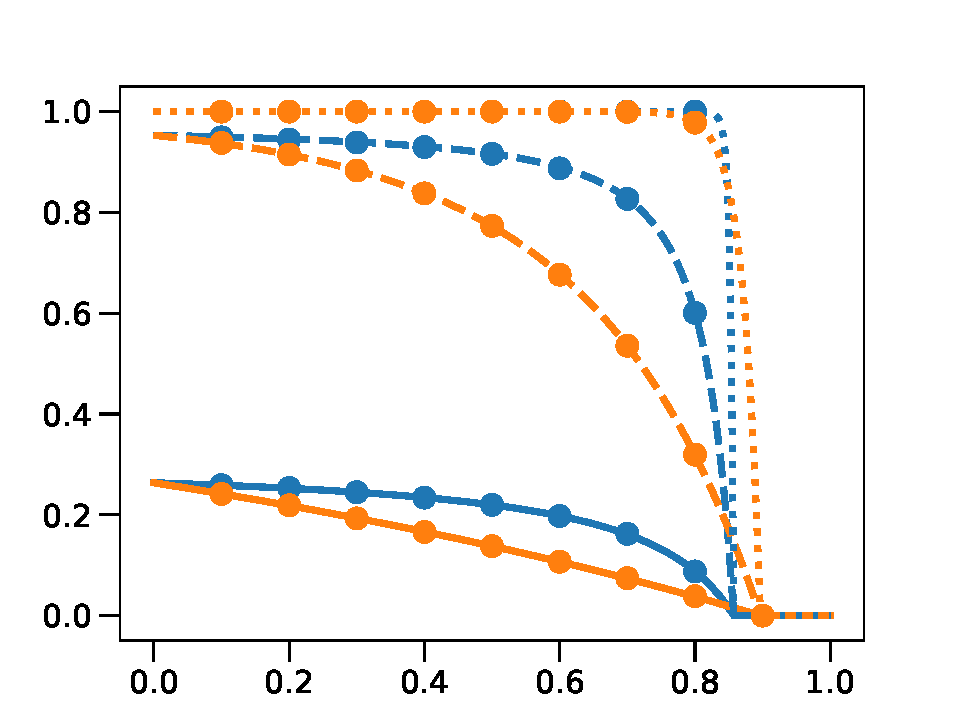
\includegraphics[scale=0.39]{fig2a_blank.pdf}};
   		\begin{scope}[x=(Bild.south east),y=(Bild.north west)]
			\node (right) at (1.5,0.5) {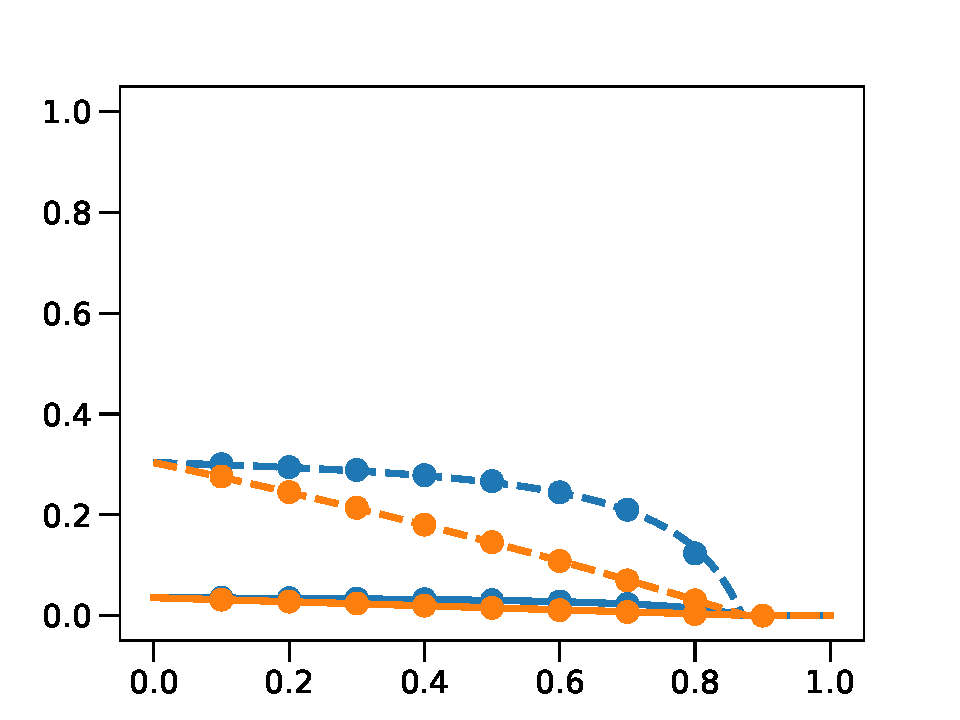
\includegraphics[scale=0.39]{fig2b_blank.pdf}}; 
			\node (right) at (0.5,-0.55) {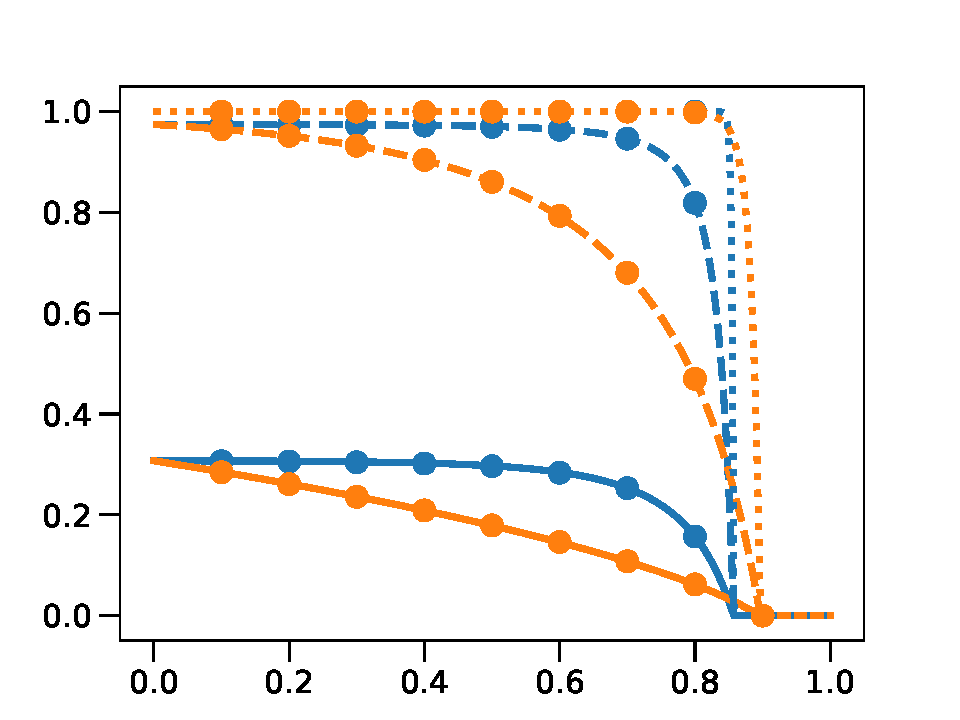
\includegraphics[scale=0.39]{figS1c_blank.pdf}};
			\node (right) at (1.5,-0.55) {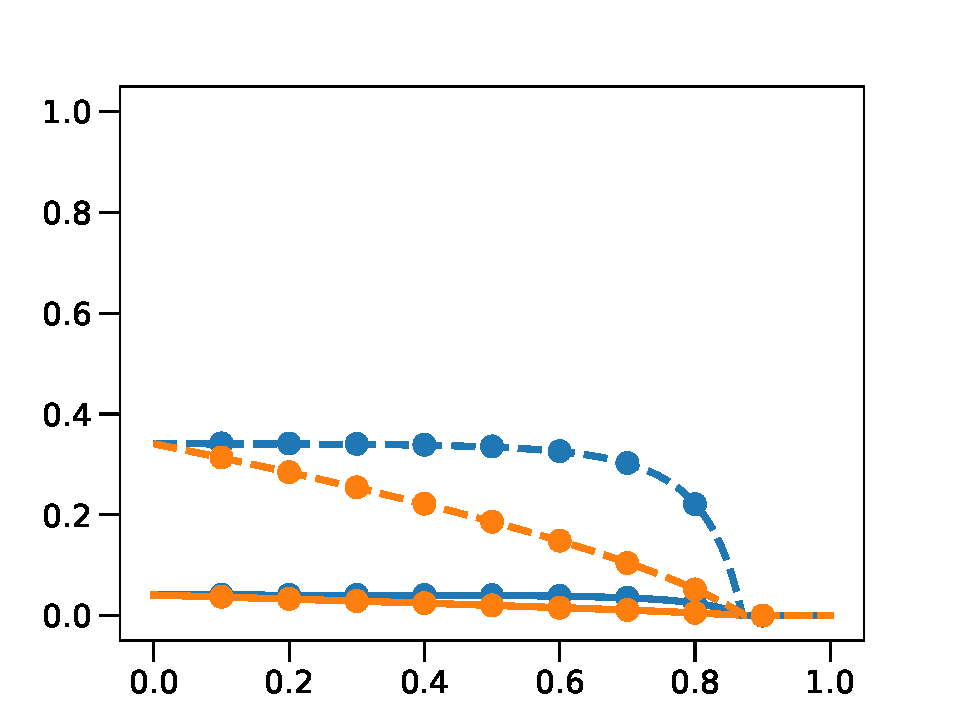
\includegraphics[scale=0.39]{figS1d_blank.pdf}};    
			  	
        	\draw (,-0.035) node {antiviral drug efficacy $\varepsilon_j$};
        	\draw (0.0,-0.) node [rotate=90] {establishment probability $\varphi$};
        	\draw (,-1.1) node {antiviral drug efficacy $\varepsilon_j$};   
        	
        	\draw (0.52,1) node {low burst size parameter set (LowN)};
        	\draw (1.51,1) node {high burst size parameter set (HighN)};     	
        	
        	\draw[black,thick] (2.1,0.6) node {\color{black} continuous};
        	\draw[black,thick] (2.1,0.525) node {\color{black} output model};  	
        	
        	\draw[black,thick] (2.1,-0.5) node {\color{black} burst model};
        	
        	\draw[black,very thick] (1.95,-0.075) -- node[right=6pt] {\color{black} $V_0=1$} (2,-0.075);
        	\draw[black,very thick,dashed] (1.95,0.025) -- node[right=6pt] {\color{black} $V_0 = 10$} (2,0.025);
        	%\draw[black,thick,dotted] (1.95,-0.15) -- node[right=6pt] {\color{black} $V_0 = 100$} (2,-0.15);
        	
        	\draw[nblue,very thick] (0.2,-1.2) -- node[right=10pt] {\color{black} reducing viral production $p$} (0.3,-1.2);
        	\draw[orange,very thick] (1.2,-1.2) -- node[right=10pt] {\color{black} reducing infectivity $\beta$} (1.3,-1.2);
    		\end{scope}
\end{tikzpicture}

\end{document}